\documentclass[../main.tex]{subfiles}
\begin{document}

\section{Notation \& Definitions}
In this section we introduce a mathematical description of the visualization pipeline where artist $A$ functions transform data of type $\Gamma(E)$ to an intermediate representation in prerendered display space of type $\Gamma(H)$:

\begin{equation}
    A: \Gamma(E) \rightarrow \Gamma(H)
    \label{eq:artist}
\end{equation}

\begin{equation}
    A: \sigma \rightarrow \rho
\end{equation}

\begin{itemize}
\item $A$ is the function that converts an instance of data $\Gamma(E)$ to an instance of a visual representation $\Gamma(H)$ 
\item $E$ is a locally trivial fiber bundle over $K$ representing data space.
\item $K$ is a triangulizable space encoding the connectivity of the observations in the data. 
\item $H$ is a fiber bundle over $S$ representing visual space
\item $S$ is a simplacial complex of triangles encoding the connectivity of the visualization of $\Gamma(E)$
\item $\sigma: K\rightarrow E$ is the data being visualized
\item $\rho: S \rightarrow H$ is the render map
\end{itemize}

When $E$ is a trivial fiber bundle $E = F \times K$, it can be assumed that all fibers $F_{k}$ over $k \in K$ are equal. Fiber bundles are product spaces of toplological spaces, which are a set of points with a set of neighborhoods for each point\cite{FiberBundle2020, rowlandFiberBundle}.

\subsection{Data Model}

We use a fiber bundle model to represent the data, as proposed by Butler 
\cite{butlerVectorBundleClassesForm1992,butlerVisualizationModelBased1989}. A fiber bundle is a structure $(E, K, \pi, F)$  consisting of topological spaces $E, K, F$ and the map from total space to base space:

\begin{equation}
    \begin{tikzcd}
        F \arrow[r, hook] & E \arrow[d, "\pi" description, bend right ] \\
                        & K \arrow[u, description, bend right]
    \end{tikzcd}
\end{equation}

where there is a bijection from $F$ to every fiber $F_k$ over point $k \in K$ in $E$ and the function $\pi: E \rightarrow K$ is the map into the $K$ quotient space of $E$. Every point in the base space $k \in K$ has a local open set neighborhood $U$ \cite{FiberBundle2020, rowlandFiberBundle}

\begin{equation}
    \begin{tikzcd}
        \pi^{-1}(U) \arrow[r, "\varphi" description] \arrow[d, "\pi" description] & U \times F \arrow[ld, "\mathrm{proj}_U"] \\
        U                                                                         &                                         
    \end{tikzcd}
\end{equation}
such that $\varphi: \pi^{-1}(U) \rightarrow U \times F$ is a homeomorphism where $\pi$ and $\mathrm{proj}_U$ both map to $U$ and the fiber over $k$ $F_k = \pi^{-1}({k \in K}) $ is homomorphic to the fiber $F$.

The section $\sigma$ is the mapping $\sigma: K\rightarrow E$ 
\begin{equation}
    \begin{tikzcd}
        F \arrow[r, hook] & E \arrow[d, "\pi" description, bend right]    \\
                          & K \arrow[u, "\sigma" description, bend right]
        \end{tikzcd}
\end{equation}

such that it is the right inverse of $\pi$
\begin{equation}
    \pi(\sigma(k)) = k \text{ for all } k \in K 
\end{equation}

In a locally trivial fiber bundle, $\sigma = K \times E$ \cite{rowlandFiberBundle,FiberBundle2020}:
\begin{equation}
\sigma(k) = (k, g(k))
\end{equation}

where the domain of $g(k)$ is $F_k$.  The space of sections over $U \subset K$ is called a sheaf and the space of all possible sections $\sigma$ of $E$ is $\Gamma(E)$. All datasets $\sigma \in \Gamma(E)$ have the same variables $F$ and connectivity $K$ but can have different values such that $\sigma_{i}\neq\sigma_{j}$.

\begin{figure}[ht]
    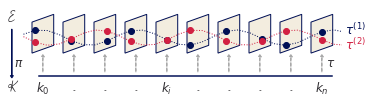
\includegraphics[width=.2\linewidth]{figures/sections/math/fiberbundle.png}
    \caption{write up some words here}
    \label{fig:fiberbundle}
\end{figure}

As illustrated by figure~\ref{fig:fiberbundle}, the vertical lines $F$ are the range of possible temperature values embedded in the total space $E$. The base space $K$ of the fiber bundle describes the connectivity of the points in $E$; in figure~\ref{fig:fiberbundle} the connectivity of the timeseries is encoded in the line representation of $K$. 

\subsubsection{Base Space $K$}

\begin{figure}[ht]
    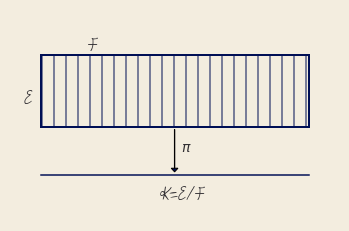
\includegraphics[width=0.4\linewidth]{figures/sections/math/k_qspace.png}
    \label{fig:kquote}
\end{figure}

$K$ is the quotient space of $E$, meaning it is the set of equivalence classes of elements $p$ in of $E$ defined via the map $\pi: E \rightarrow K$ that sends each point $p \in E$ to its equivalence class in $[p] \in K$ \cite{QuotientSpaceTopology2020,QuotientSpaceTopology2020}. As shown in figure~\ref{fig:kquote}, the fibers $F$ divide $E$ into smaller spaces consisisting of $F$ and an open set neighborhood around $F$. This subdivision is projected down to the toplology $\tau_k$

\begin{equation}
\tau_K = \{U\subseteqq K: \{p \in E: [p] \in U\}\in \tau_E\}
\end{equation}

where $[p] \in U$ is the point $k \in K$ with an open set around it that has an open  preimage in $E$ under the surjective map $\pi: p \rightarrow [p]$. 


\begin{figure}[ht]
    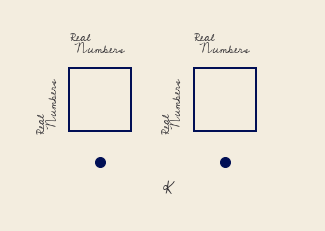
\includegraphics[width=0.2\linewidth]{figures/sections/math/temp_1k.png}
    %% add box around neighboring P and Map
    \label{fig:k_data}
\end{figure}
\begin{figure}[ht]
    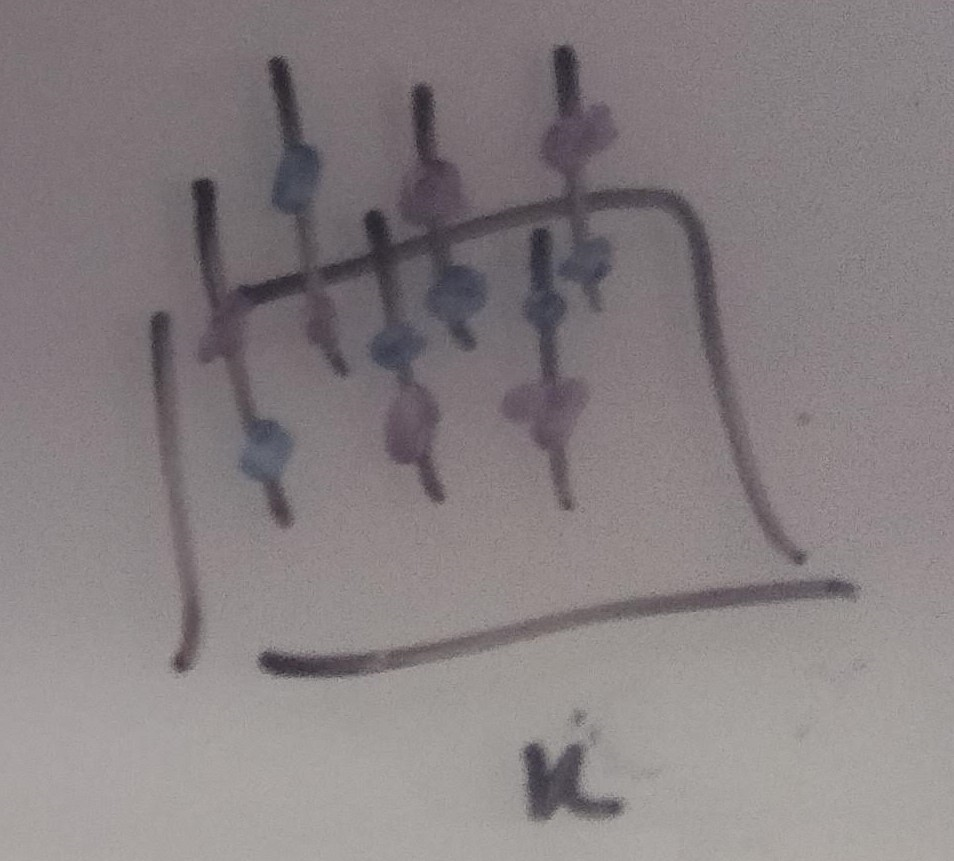
\includegraphics[width=0.2\linewidth]{figures/sections/math/temp_2k.png}
\end{figure}

We use $K$ to encode the connectivity of the points $p$. In figure~\ref{fig:k_data}, there is only one data field in $p$, temperature, but the points $p$ are connected differently. In a timeseries, the temperature $p$ at time $t$ is dependent on the value at $p_{t-1}$ and $p_{t+1}$ is dependent on the value in $p_t$; this connectivity is expressed as a one dimensional $K$ where $K$ is the number line. In the case of the map, every point $p$ is dependent on its nearest neighbors on the plane, and one way to express this is by encoding $K$ as a plane. $K$ does not know the time or latitude or longitude of the point - those are metadata variables potentially encoded in $p$ because they are ways of describing the connectivity rather than the connectivity itself. The mapping $sigma: K \rightarrow E$ provides the binding between the key on $K$ and the value $p$ in $E$ \cite{munznerChDataAbstraction}.

\subsubsection{Fiber Space $F$}
Spivak models the fiber space $F$ as schema and the data as sheafs (localized $\sigma$ functions) on the schema \cite{spivakSIMPLICIALDATABASES}. He defines the type specification 
\begin{equation}
\pi: U \rightarrow DT
\end{equation}

where $DT$ is the set of data types (as identified by their names) and $U$ is the disjoint set of all possible objects $x$ of all types in $DT$. This means that for each type $T\in DT$, the preimage $\pi^{-1}(T)\subset U $ is the domain of $T$, and $x \in \pi^{1}(T)\subset U$ is an object of type $T$. Spivak then defines a schema $(C, \sigma)$ of type $\pi$, where $\pi$ is the universe of all types, such that 
\begin{equation}
\sigma: C \rightarrow DT
\end{equation}
where $C$ is the finite set of names of data fields in $E$. The set of all values restricted to the datatypes in $DT$ is $U_{\sigma}$

\begin{equation}
    \begin{tikzcd}
            U_{\sigma} \arrow[d, "\pi_{\sigma}" description] \arrow[r] & U \arrow[d, "\pi" description] \\
            C \arrow[r, "\sigma" description]                          & DT                            
    \end{tikzcd}
\end{equation}
The pullback $U_{\sigma} \coloneqq \sigma^{-1}(U)$ restricts $U$ to the datatypes of the fields in $C$ such that $U_{\sigma}$ is the fiber product $U \times_{DT} C$, and the pullback $\pi_{\sigma}:U_{\sigma} \rightarrow C$ defines a domain bundle $U_{\sigma}$ over $C$ induced by $\sigma$.




In the fiber bundle, $F$ is the cartesian product of all sets in the disjoint union $U_{\sigma}$

The record function is the sigma function


\begin{figure}[ht]
    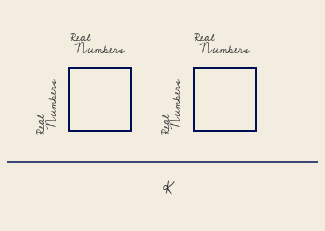
\includegraphics[width=0.2\linewidth]{figures/sections/math/temp_2f.png}
    \label{fig:}
\end{figure}
\begin{figure}[ht]
    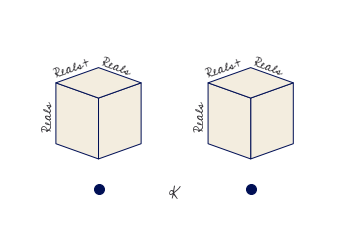
\includegraphics[width=0.2\linewidth]{figures/sections/math/temp_3f.png}
\end{figure}


The fibers $F$ are a topological space embedded in $E$ on which lie the set of all possible values. For example, if $F$ is the interval $[0, 1]$, then $g(k)$ from equation~\ref{eq:sigma} returns a single measurement $x$ in the interval $F$:
\begin{equation}
    \label{eg:goff}
    g(k) = x, \text{ where } 0\leq x \leq 1
\end{equation}

The fiber in figure~\ref{fig:temp} is the space of possible temperature values in $\circ$ celsius, ranging from [start, end], similar to the interval $F$ in equation~\ref{eg:goff}. F can be any number of dimensions, for example in figure~\ref{fig:temp_time} time is encoded as a second dimension. Given:
\begin{itemize}
\item interval of all possible temperature values $[T_{min}, T_{max}]$ 
\item interval of all possible time values $[t_{min}, t_{max}]$
\end{itemize}

then $F$ is the cross product $F= [T_{min}, T_{max}] \times [t_{min}, t_{max}]$, and $g(k)$ listed in equation~\ref{eq:sigma} is:

\begin{equation}
g(k) = (x_0, x_1) \text{ where } x_0 \in [T_{min}, T_{max}], x_1 \in [t_{min}, t_{max}]
\end{equation}


% datetime type, columns = start, end 

% schema is ordered list of Column, type is approx F, U cross C over sigma, 
% space of rows/records f:k -> r, sigma:k -> r, is the table function (dataframe as instance)
When $E$ is trivial, then we can decompose $E$ so that each $E$ 


\subsubsection{Subset}
$\Gamma(E)$ is the space of all points in $F$ returned by $\sigma$; therefore the points being visualized in a streaming or animation example can be considered a subset that lives on base space $U \subset K$ with the same fiber $F$
\begin{equation}
    \begin{tikzcd}
        \iota^\ast E \arrow[r, hook] \arrow[d]                                                                       & E \arrow[d, bend right]                       \\
        U \arrow[r, "\iota" description, hook] \arrow[u, "\iota^\ast \sigma" description, bend right, shift right=2] & K \arrow[u, "\sigma" description, bend right]
    \end{tikzcd}    
\end{equation}
where $\iota^*E$ and $\iota^*\sigma$ are $E$ and $\sigma$ restricted to points $k \in U \subset K$.   


\subsection{Prerender Space}
\label{sec:display}

% preamble type intro to displays, examples - displays can include screen, 3D printer, sphereical display, H is the total space of the screen. 11
\begin{figure}[h]
    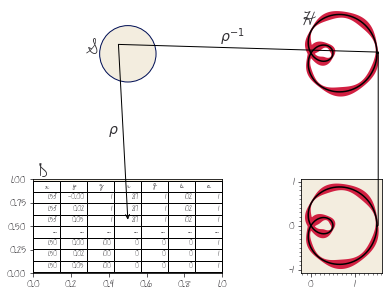
\includegraphics[width=.4\linewidth]{figures/sections/math/render.png}
    \caption{}
    \label{fig:render}
\end{figure}

A physical display space can be thought of sets of $\mathbb{R}^{7}$ tuples, where 
\begin{equation}
    \mathbb{R}^{7} = \{X, Y, Z, R, G, B, A\}
\end{equation}

and the sets correspond to the sections on $\S$, which is the topology of the output of the artist $A$. The space $H$ is a total space representing the predisplay space, with a fiber of $\mathbb{R}^7$ and a base space of $\S$:
\begin{equation}
    \begin{tikzcd}
        \mathbb{R}^{7} \arrow[r, hook] & H \arrow[d, "\pi" description, bend right] \\
                                    & S \arrow[u, "\rho" description, bend right] 
    \end{tikzcd}
\end{equation}


In the case of 2D screens, the predisplay space is a trivial fiber bundle $H=\mathbb{R}^{7}\times S$. As illustrated in figure~\ref{fig:render}, a region on the screen defined by the corners $(x_1, y_1)$ and $(x_2, y_2)$ maps into a region on a 2-simplex in $S$ defined by $(\alpha_1, \beta_1)$ and $(\alpha_2, \beta_2)$. The function on the simplex $f$ returns the (R, G, B, A) value for that $(\alpha, \beta)$ pair. For a region, 

\begin{equation*}
\rho(S) = \int_{\alpha_1}^{\alpha_2}\int_{\beta_1}^{\beta_2}\int_{z_1}^{z_2}{R, G, B, A}  
\end{equation*}

where the R,G,B,A values are derived from the how the data values are mapped to visual characteristics. The z component of the mapping to $\mathbb{R}^7$ is moved to the integration because this is a trivial space representing a 2D screen; $\rho$ varies depending on $H$. 

%%%pho is paramterized over alpha, beta, which is obtained via pullback lookup from (Hx,Hy)-?(alpha, beta)

\subsection{Artist}
%% include some words about motivation 
\begin{equation}
    A: \Gamma(E) \rightarrow \Gamma(H)
\end{equation}

\subsubsection{Screen to Data}
%%diagram: [data] -Tau->[RGVXYZ]
%%%            \ /\ / 
\begin{equation}
    \begin{tikzcd}
        E \arrow[d, "\pi" description] & H \arrow[d, "\pi" description]                                                 \\
        K \arrow[u, "\sigma" description, bend right] & S \arrow[l, "\xi" description] \arrow[u, "\rho" description, bend right]
    \end{tikzcd}
\end{equation}
The pullback $\xi$ on $S \rightarrow K$ means that the values in $E$ can be directly mapped to a simplex in $S$, which means there's a mapping from screen space back to the values. 
\begin{equation}
    \begin{tikzcd}
        \xi E \arrow[rr, "\tau" description] \arrow[rd, "\xi \sigma" description, bend right] &     & H \arrow[ld] \\
        & S \arrow[lu, bend right] &             
    \end{tikzcd}
\end{equation}

\subsubsection{Marks}
%% diagram of connected components/line thing 11-19-20 notes
Bertin describes a location on the plane as the signifying characteristic of a point, measurable length as the signifying characteristic of a line, and measurable size as the signifying characteristic of an area and that in display (pixel) space these are marks \cite{bertinIIPropertiesGraphic2011,carpendaleVisualRepresentationSemiology}. 
\begin{equation}
\begin{tikzcd}
    H \arrow[r, shift left] & S \arrow[l, "\rho(\xi^{-1}(J))", shift left] \arrow[rr, "\xi(s)", shift left] &  & J_{k} =  \{j \in K| \exists \Gamma \text{ s.t. } \Gamma(0)=k \text{ and }\Gamma(1)=j\} \arrow[ll, "\xi^{-1}(J)", shift left]
\end{tikzcd}
\label{eq:mark}
\end{equation}

Each point $s$ in the display space $H$, the mark it belongs to can be found by mapping $s$ back to $K$ via the lookup on S described in section~\ref{sec:display} then taking $\xi(s)$ back to a point on $k \in K$ which lies on the connected component $J \subset K$. To got back to the display space $H$  from the simplacial complex $J$ of the signifier implanted in the mark, the inverse image of $J \in S, \xi^{-1}(J)$ is pushed back to $S$, and then  $\rho(\xi^{-1}(J))$ maps it into $R^{7}$. 



\subsubsection{Channels}
Acts on different parts of F, types means measurement groups , can be broken out so 
%%tau(E_{u} in E)
Tau can preserves the measurement type properties (group scales)

%%The measurement spaces $X$ are each variables and have the properties of measurement scales, such as Steven's nominal, ordinal, interval, and ratio \cite{stevensTheoryScalesMeasurement1946}. Stevens talks about measurements and this is how we define it here:.... can check symmatry under stevens via carry through on tau

Tau is fully flexible and can do whatever; knows about fiber \& neighborhood of fiber. Can in theory approximate hatching/dashing/etc can be approximated w/ functions and neighborhood of k. 

%%hatches can either grow the R space or function 

\subsubsection{Visual Idioms: Equivalance class of artists}
Two artists are equivalent when given data containers $\Gamma(E)$ of the same type, they output the same type of prerender $\Gamma(S)$:
\begin{equation}
    \begin{tikzcd}
        A_{\tau_2}: \arrow[d, shift right=2] & \Gamma(E) \arrow[r] & \Gamma(H) &                                                \\
        A_{\tau_1}: \arrow[u, shift right]   & \Gamma(E) \arrow[r] & \Gamma(H) 
    \end{tikzcd}
\end{equation}

\end{document}